\documentclass{article}
\usepackage{bookmark}
\usepackage{color}
\usepackage{listings}
\usepackage{amsmath}
\usepackage{hyperref}
\usepackage{listings}
\usepackage{xcolor}
\usepackage{graphicx}
\usepackage{amsfonts}
\definecolor{dkgreen}{rgb}{0,0.6,0}
\definecolor{gray}{rgb}{0.5,0.5,0.5}
\definecolor{mauve}{rgb}{0.58,0,0.82}

\lstset{
  basicstyle=\footnotesize, 
  numbers=left, 
  numberstyle=\tiny\color{gray}, 
  stepnumber=1,
  numbersep=5pt, 
  backgroundcolor=\color{white},
  showspaces=false,
  showstringspaces=false,
  showtabs=false,
  frame=shadowbox,
  rulecolor=\color{black},
  tabsize=2,
  captionpos=b,
  breaklines=true, 
  breakatwhitespace=false, 
  title=\lstname,
  keywordstyle=\color{blue},
  commentstyle=\color{dkgreen},
  escapeinside={\%*}{*)}, 
  morekeywords={*,...} 
}

\begin{document}
\begin{itemize}
\item {\bf Ex. 1}\\
{\noindent 1. For first fit, it should be 20KB for (i), 10KB for (ii) and 18KB for (iii).} 

For best fit, it should be 12KB for (i), 10KB for (ii) and 9KB for (iii).

For quick fit, it should be 12KB for (i), 10KB for (ii) and 9KB for (iii).\\

{\noindent 2. It should be $10k/(10k+n)$\\}

{\noindent 3. It should be 01101110 for C0, 01001001 for C1, 00110111 for C2 and 10001011 for C3\\}

\item {\bf EX. 2}\\
The following things comes from "Page Table" page from Wikipedia: \url{https://en.wikipedia.org/wiki/Page_table}

The inverted page table (IPT) is best thought of as an off-chip extension of the TLB which uses normal system RAM. Unlike a true page table, it is not necessarily able to hold all current mappings. The OS must be prepared to handle misses, just as it would with a MIPS-style software-filled TLB.

The IPT combines a page table and a frame table into one data structure. At its core is a fixed-size table with the number of rows equal to the number of frames in memory. If there are 4000 frames, the inverted page table has 4000 rows. For each row there is an entry for the virtual page number (VPN), the physical page number (not the physical address), some other data and a means for creating a collision chain, as we will see later.

To search through all entries of the core IPT structure is inefficient, and a hash table may be used to map virtual addresses (and address space/PID information if need be) to an index in the IPT - this is where the collision chain is used. This hash table is known as a hash anchor table. The hashing function is not generally optimized for coverage - raw speed is more desirable. Of course, hash tables experience collisions. Due to this chosen hashing function, we may experience a lot of collisions in usage, so for each entry in the table the VPN is provided to check if it is the searched entry or a collision.

In searching for a mapping, the hash anchor table is used. If no entry exists, a page fault occurs. Otherwise, the entry is found. Depending on the architecture, the entry may be placed in the TLB again and the memory reference is restarted, or the collision chain may be followed until it has been exhausted and a page fault occurs.

A virtual address in this schema could be split into two, the first half being a virtual page number and the second half being the offset in that page.

A major problem with this design is poor cache locality caused by the hash function. Tree-based designs avoid this by placing the page table entries for adjacent pages in adjacent locations, but an inverted page table destroys spatial locality of reference by scattering entries all over. An operating system may minimize the size of the hash table to reduce this problem, with the trade-off being an increased miss rate.

There is normally one hash table, contiguous in physical memory, shared by all processes. A per-process identifier is used to disambiguate the pages of different processes from each other. It is somewhat slow to remove the page table entries of a given process; the OS may avoid reusing per-process identifier values to delay facing this. Alternatively, per-process hash tables may be used, but they are impractical because of memory fragmentation, which requires the tables to be pre-allocated.

Inverted page tables are used for example on the PowerPC, the UltraSPARC and the IA-64 architecture.

The inverted page table keeps a listing of mappings installed for all frames in physical memory. However, this could be quite wasteful. Instead of doing so, we could create a page table structure that contains mappings for virtual pages. It is done by keeping several page tables that cover a certain block of virtual memory. For example, we can create smaller 1024-entry 4K pages that cover 4M of virtual memory.

This is useful since often the top-most parts and bottom-most parts of virtual memory are used in running a process - the top is often used for text and data segments while the bottom for stack, with free memory in between. The multilevel page table may keep a few of the smaller page tables to cover just the top and bottom parts of memory and create new ones only when strictly necessary.

Now, each of these smaller page tables are linked together by a master page table, effectively creating a tree data structure. There need not be only two levels, but possibly multiple ones.

A virtual address in this schema could be split into three parts: the index in the root page table, the index in the sub-page table, and the offset in that page.

Multilevel page tables are also referred to as hierarchical page tables.



\item {\bf Ex. 4}\\
{\noindent 1. The files related are all in the directory minix/servers/vm}\\

{\noindent 2. It should be 4096}

{\noindent 3. It is got from the file minix/servers/vm/pt.h}

\newpage

\begin{figure}[h]
    \centering
    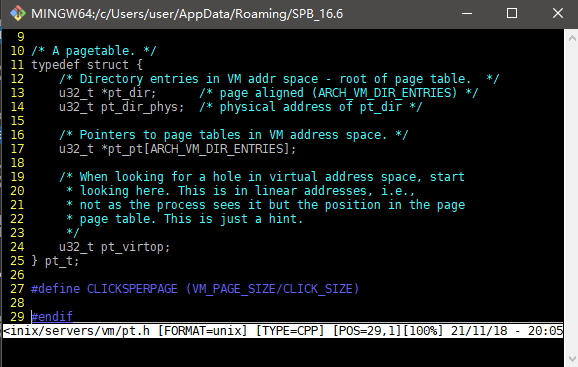
\includegraphics[scale=0.5]{1.png}
\end{figure}

{\noindent 4. It is got from the file minix/servers/vm/proto.h}

\begin{figure}[h]
    \centering
    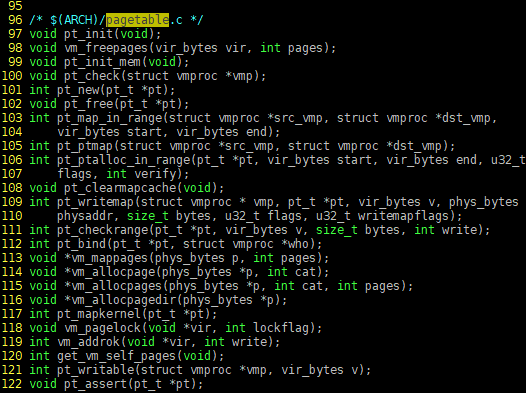
\includegraphics[scale=0.5]{2.png}
\end{figure}

{\noindent }
\item {\bf Ex. 5}\\

{\noindent 1. This should be done using count\_lock. Use this to access the counter and change it for reading.}

\begin{lstlisting}[language=C]
void read_lock(){
    down(count_lock);
    if (counter==0) down(db_lock);
    counter++;
    up(count_lock);      
}

void read_lock(){
    down(count_lock);
    if (counter==1) up(db_lock);
    counter--;
    up(count_lock);      
}


\end{lstlisting}
{\noindent 2. It means that the writer cannot find time to write on the db, bercause readers are coming continuously.\\}

{\noindent 3. This can be done by adding down(read\_lock) and up(read\_lock) in both read\_lock() and write\_lock()\\}

{\noindent 4. No as the writer still has higher priority, so the problem should not be regarded as solved.}

\item {\bf Ex. 6}\\
The following things comes from "Dirty COW" page from Wikipedia: \url{https://en.wikipedia.org/wiki/Dirty_COW
}

Dirty COW (Dirty copy-on-write) is a computer security vulnerability for the Linux kernel that affects all Linux-based operating systems including Android. It is a local privilege escalation bug that exploits a race condition in the implementation of the copy-on-write mechanism in the kernel's memory-management subsystem. The vulnerability was discovered by Phil Oester. Because of the race condition, with the right timing, a local attacker can exploit the copy-on-write mechanism to turn a read-only mapping of a file into a writable mapping. Although it is a local privilege escalation, remote attackers can use it in conjunction with other exploits that allow remote execution of non-privileged code to achieve remote root access on a computer. The attack itself does not leave traces in the system log.

The vulnerability has the Common Vulnerabilities and Exposures designation CVE-2016-5195.Dirty COW (Dirty copy-on-write) is a computer security vulnerability for the Linux kernel that affects all Linux-based operating systems including Android. It is a local privilege escalation bug that exploits a race condition in the implementation of the copy-on-write mechanism in the kernel's memory-management subsystem. The vulnerability was discovered by Phil Oester.Because of the race condition, with the right timing, a local attacker can exploit the copy-on-write mechanism to turn a read-only mapping of a file into a writable mapping. Although it is a local privilege escalation, remote attackers can use it in conjunction with other exploits that allow remote execution of non-privileged code to achieve remote root access on a computer. The attack itself does not leave traces in the system log.

The vulnerability has the Common Vulnerabilities and Exposures designation CVE-2016-5195.[3] Dirty Cow was one of the first security issues transparently fixed in Ubuntu by the Canonical Live Patch service.[4]

It has been demonstrated that the vulnerability can be utilized to root any Android device up to Android version  Dirty Cow was one of the first security issues transparently fixed in Ubuntu by the Canonical Live Patch service.

It has been demonstrated that the vulnerability can be utilized to root any Android device up to Android version 


\end{itemize}
\end{document}